\documentclass{standalone}
\usepackage{tikz}
\usetikzlibrary{patterns, positioning}
\usepackage[sfdefault]{ClearSans} %% option 'sfdefault' activates Clear Sans as the default text font
\usepackage[T1]{fontenc}

\begin{document}
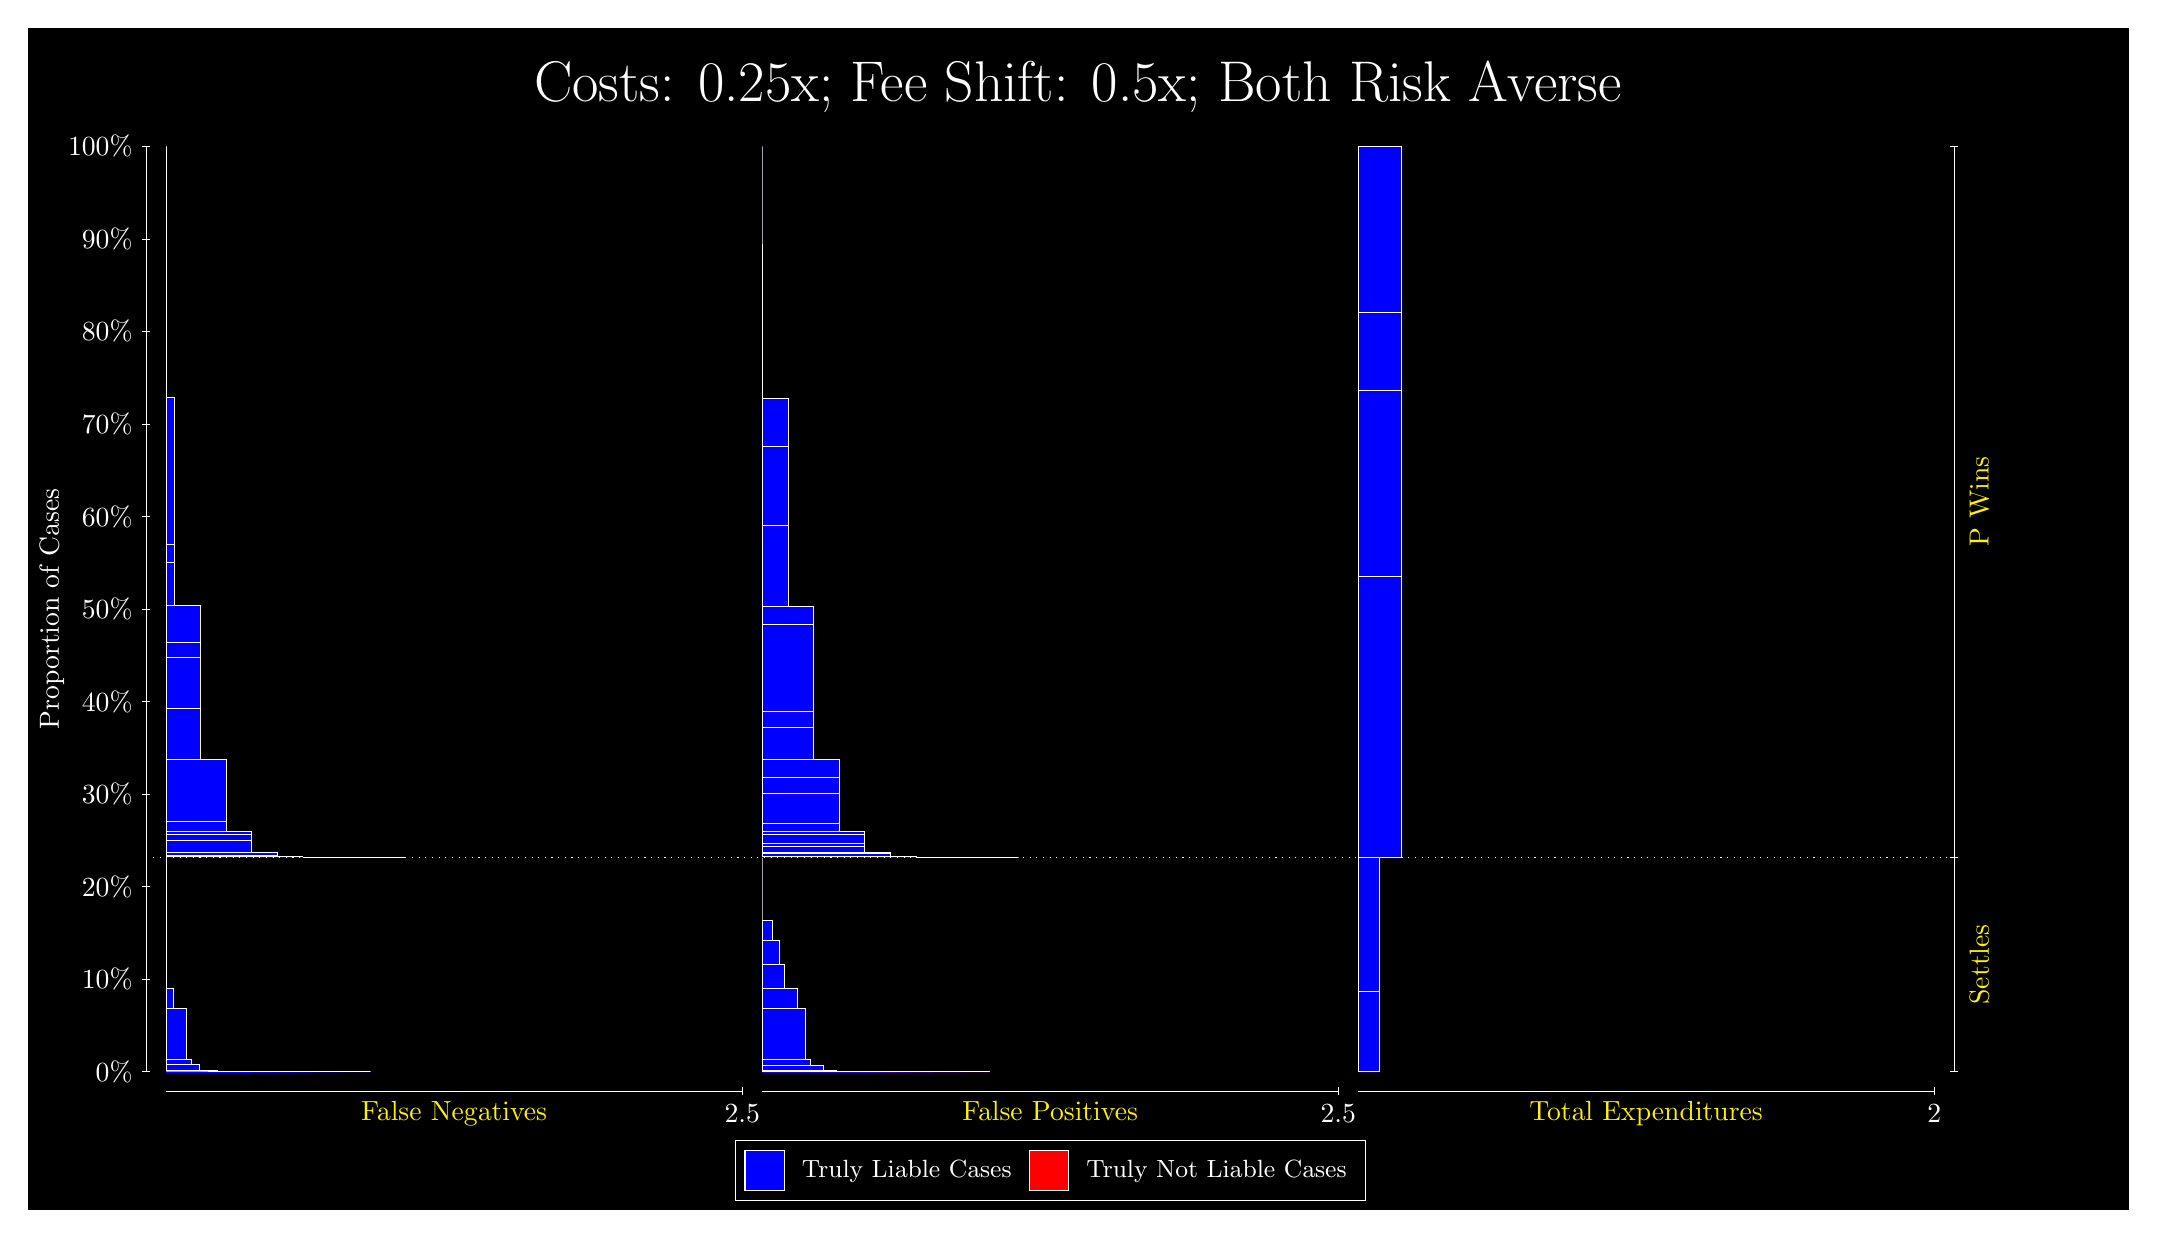
\begin{tikzpicture}
\draw[fill=black] (0,0) rectangle (26.667,15);
\draw[text=white] (0,13.5) rectangle (26.667,15) node[midway] {\huge Costs: 0.25x; Fee Shift: 0.5x; Both Risk Averse};
\draw[white, very thin] (1.5,1.75) -- (1.5,13.5);
\node[rotate=90, text=white, anchor=center] at (0.3, 7.625) {Proportion of Cases};
\draw[white, very thin] (1.45,1.75) -- (1.55,1.75);
\node[text=white, anchor=east] at (1.45, 1.75) {0\%};
\draw[white, very thin] (1.45,2.925) -- (1.55,2.925);
\node[text=white, anchor=east] at (1.45, 2.925) {10\%};
\draw[white, very thin] (1.45,4.1) -- (1.55,4.1);
\node[text=white, anchor=east] at (1.45, 4.1) {20\%};
\draw[white, very thin] (1.45,5.275) -- (1.55,5.275);
\node[text=white, anchor=east] at (1.45, 5.275) {30\%};
\draw[white, very thin] (1.45,6.45) -- (1.55,6.45);
\node[text=white, anchor=east] at (1.45, 6.45) {40\%};
\draw[white, very thin] (1.45,7.625) -- (1.55,7.625);
\node[text=white, anchor=east] at (1.45, 7.625) {50\%};
\draw[white, very thin] (1.45,8.8) -- (1.55,8.8);
\node[text=white, anchor=east] at (1.45, 8.8) {60\%};
\draw[white, very thin] (1.45,9.975) -- (1.55,9.975);
\node[text=white, anchor=east] at (1.45, 9.975) {70\%};
\draw[white, very thin] (1.45,11.15) -- (1.55,11.15);
\node[text=white, anchor=east] at (1.45, 11.15) {80\%};
\draw[white, very thin] (1.45,12.325) -- (1.55,12.325);
\node[text=white, anchor=east] at (1.45, 12.325) {90\%};
\draw[white, very thin] (1.45,13.5) -- (1.55,13.5);
\node[text=white, anchor=east] at (1.45, 13.5) {100\%};

\draw[white, very thin] (24.457,1.75) -- (24.457,13.5);
\draw[white, very thin] (24.407,1.75) -- (24.507,1.75);
\node[anchor=west] at (24.407, 1.75) {};
\draw[white, very thin] (24.407,4.4726) -- (24.507,4.4726);
\node[anchor=west] at (24.407, 4.4726) {};
\draw[white, very thin] (24.407,13.5) -- (24.507,13.5);
\node[anchor=west] at (24.407, 13.5) {};

\draw[white, very thin, fill=blue] (1.75,1.75) rectangle (4.3482,1.75);
\draw[white, very thin, fill=blue] (1.75,1.75) rectangle (4.0229,1.75);
\draw[white, very thin, fill=blue] (1.75,1.75) rectangle (3.9091,1.75);
\draw[white, very thin, fill=blue] (1.75,1.75) rectangle (3.6976,1.75);
\draw[white, very thin, fill=blue] (1.75,1.75) rectangle (3.5838,1.75);
\draw[white, very thin, fill=blue] (1.75,1.75) rectangle (3.4699,1.75);
\draw[white, very thin, fill=blue] (1.75,1.75) rectangle (3.3723,1.75);
\draw[white, very thin, fill=blue] (1.75,1.75) rectangle (3.2585,1.75);
\draw[white, very thin, fill=blue] (1.75,1.75) rectangle (3.1772,1.75);
\draw[white, very thin, fill=blue] (1.75,1.75) rectangle (3.1447,1.75);
\draw[white, very thin, fill=blue] (1.75,1.75) rectangle (3.0471,1.75);
\draw[white, very thin, fill=blue] (1.75,1.75) rectangle (2.9332,1.75);
\draw[white, very thin, fill=blue] (1.75,1.75) rectangle (2.8519,1.75);
\draw[white, very thin, fill=blue] (1.75,1.75) rectangle (2.8194,1.7503);
\draw[white, very thin, fill=blue] (1.75,1.7503) rectangle (2.738,1.7503);
\draw[white, very thin, fill=blue] (1.75,1.7503) rectangle (2.7218,1.7503);
\draw[white, very thin, fill=blue] (1.75,1.7503) rectangle (2.6079,1.7503);
\draw[white, very thin, fill=blue] (1.75,1.7503) rectangle (2.5266,1.7503);
\draw[white, very thin, fill=blue] (1.75,1.7503) rectangle (2.4941,1.7576);
\draw[white, very thin, fill=blue] (1.75,1.7576) rectangle (2.4128,1.7576);
\draw[white, very thin, fill=blue] (1.75,1.7576) rectangle (2.3965,1.7624);
\draw[white, very thin, fill=blue] (1.75,1.7624) rectangle (2.2827,1.7626);
\draw[white, very thin, fill=blue] (1.75,1.7626) rectangle (2.2013,1.7626);
\draw[white, very thin, fill=blue] (1.75,1.7626) rectangle (2.1688,1.8358);
\draw[white, very thin, fill=blue] (1.75,1.8358) rectangle (2.0875,1.8358);
\draw[white, very thin, fill=blue] (1.75,1.8358) rectangle (2.0712,1.9027);
\draw[white, very thin, fill=blue] (1.75,1.9027) rectangle (2.0062,2.5534);
\draw[white, very thin, fill=blue] (1.75,2.5534) rectangle (1.9574,2.5556);
\draw[white, very thin, fill=blue] (1.75,2.5556) rectangle (1.876,2.5556);
\draw[white, very thin, fill=blue] (1.75,2.5556) rectangle (1.8435,2.8061);
\draw[white, very thin, fill=blue] (1.75,2.8061) rectangle (1.7622,2.8061);
\draw[white, very thin, fill=red] (1.75,2.8061) rectangle (1.75,2.8061);
\draw[white, very thin, fill=blue] (1.75,2.8061) rectangle (1.75,4.4726);
\draw[white, very thin, fill=blue] (1.75,4.4726) rectangle (4.7873,4.4726);
\draw[white, very thin, fill=blue] (1.75,4.4726) rectangle (4.462,4.4726);
\draw[white, very thin, fill=blue] (1.75,4.4726) rectangle (4.462,4.4726);
\draw[white, very thin, fill=blue] (1.75,4.4726) rectangle (4.1368,4.4726);
\draw[white, very thin, fill=blue] (1.75,4.4726) rectangle (3.8115,4.4727);
\draw[white, very thin, fill=blue] (1.75,4.4727) rectangle (3.8115,4.4731);
\draw[white, very thin, fill=blue] (1.75,4.4731) rectangle (3.4862,4.4783);
\draw[white, very thin, fill=blue] (1.75,4.4783) rectangle (3.4862,4.4796);
\draw[white, very thin, fill=blue] (1.75,4.4796) rectangle (3.1609,4.4889);
\draw[white, very thin, fill=blue] (1.75,4.4889) rectangle (3.1609,4.4987);
\draw[white, very thin, fill=blue] (1.75,4.4987) rectangle (3.1609,4.5323);
\draw[white, very thin, fill=blue] (1.75,4.5323) rectangle (2.8356,4.6849);
\draw[white, very thin, fill=blue] (1.75,4.6849) rectangle (2.8356,4.7647);
\draw[white, very thin, fill=blue] (1.75,4.7647) rectangle (2.8356,4.804);
\draw[white, very thin, fill=blue] (1.75,4.804) rectangle (2.5103,4.9263);
\draw[white, very thin, fill=blue] (1.75,4.9263) rectangle (2.5103,5.7176);
\draw[white, very thin, fill=blue] (1.75,5.7176) rectangle (2.1851,6.3695);
\draw[white, very thin, fill=blue] (1.75,6.3695) rectangle (2.1851,7.011);
\draw[white, very thin, fill=blue] (1.75,7.011) rectangle (2.1851,7.2061);
\draw[white, very thin, fill=blue] (1.75,7.2061) rectangle (2.1851,7.6713);
\draw[white, very thin, fill=blue] (1.75,7.6713) rectangle (1.8598,8.2234);
\draw[white, very thin, fill=blue] (1.75,8.2234) rectangle (1.8598,8.4404);
\draw[white, very thin, fill=blue] (1.75,8.4404) rectangle (1.8598,10.309);
\draw[white, very thin, fill=red] (1.75,10.309) rectangle (1.75,10.309);
\draw[white, very thin, fill=blue] (1.75,10.309) rectangle (1.75,13.5);
\draw[white, very thin, fill=red] (9.3189,1.75) rectangle (12.21,1.75);
\draw[white, very thin, fill=blue] (9.3189,1.75) rectangle (12.21,1.75);
\draw[white, very thin, fill=blue] (9.3189,1.75) rectangle (11.885,1.75);
\draw[white, very thin, fill=blue] (9.3189,1.75) rectangle (11.559,1.75);
\draw[white, very thin, fill=red] (9.3189,1.75) rectangle (11.478,1.75);
\draw[white, very thin, fill=blue] (9.3189,1.75) rectangle (11.478,1.75);
\draw[white, very thin, fill=blue] (9.3189,1.75) rectangle (11.234,1.75);
\draw[white, very thin, fill=blue] (9.3189,1.75) rectangle (11.153,1.75);
\draw[white, very thin, fill=red] (9.3189,1.75) rectangle (11.039,1.75);
\draw[white, very thin, fill=blue] (9.3189,1.75) rectangle (11.039,1.75);
\draw[white, very thin, fill=blue] (9.3189,1.75) rectangle (10.909,1.75);
\draw[white, very thin, fill=blue] (9.3189,1.75) rectangle (10.827,1.75);
\draw[white, very thin, fill=red] (9.3189,1.75) rectangle (10.746,1.75);
\draw[white, very thin, fill=blue] (9.3189,1.75) rectangle (10.746,1.7502);
\draw[white, very thin, fill=blue] (9.3189,1.7502) rectangle (10.714,1.7502);
\draw[white, very thin, fill=blue] (9.3189,1.7502) rectangle (10.583,1.7504);
\draw[white, very thin, fill=blue] (9.3189,1.7504) rectangle (10.502,1.7504);
\draw[white, very thin, fill=blue] (9.3189,1.7504) rectangle (10.421,1.7562);
\draw[white, very thin, fill=blue] (9.3189,1.7562) rectangle (10.388,1.7562);
\draw[white, very thin, fill=red] (9.3189,1.7562) rectangle (10.307,1.7562);
\draw[white, very thin, fill=blue] (9.3189,1.7562) rectangle (10.307,1.7564);
\draw[white, very thin, fill=blue] (9.3189,1.7564) rectangle (10.258,1.7634);
\draw[white, very thin, fill=blue] (9.3189,1.7634) rectangle (10.177,1.7634);
\draw[white, very thin, fill=blue] (9.3189,1.7634) rectangle (10.095,1.8322);
\draw[white, very thin, fill=blue] (9.3189,1.8322) rectangle (10.063,1.8322);
\draw[white, very thin, fill=blue] (9.3189,1.8322) rectangle (9.9816,1.8343);
\draw[white, very thin, fill=blue] (9.3189,1.8343) rectangle (9.9328,1.9059);
\draw[white, very thin, fill=red] (9.3189,1.9059) rectangle (9.8678,1.9059);
\draw[white, very thin, fill=blue] (9.3189,1.9059) rectangle (9.8678,2.5564);
\draw[white, very thin, fill=blue] (9.3189,2.5564) rectangle (9.8515,2.5564);
\draw[white, very thin, fill=blue] (9.3189,2.5564) rectangle (9.7702,2.8049);
\draw[white, very thin, fill=blue] (9.3189,2.8049) rectangle (9.7377,2.8049);
\draw[white, very thin, fill=blue] (9.3189,2.8049) rectangle (9.6563,2.8097);
\draw[white, very thin, fill=blue] (9.3189,2.8097) rectangle (9.6076,3.1141);
\draw[white, very thin, fill=blue] (9.3189,3.1141) rectangle (9.5425,3.4165);
\draw[white, very thin, fill=blue] (9.3189,3.4165) rectangle (9.5262,3.4165);
\draw[white, very thin, fill=blue] (9.3189,3.4165) rectangle (9.4449,3.667);
\draw[white, very thin, fill=blue] (9.3189,3.667) rectangle (9.4124,3.667);
\draw[white, very thin, fill=blue] (9.3189,3.667) rectangle (9.3311,3.6692);
\draw[white, very thin, fill=blue] (9.3189,3.6692) rectangle (9.3189,4.4726);
\draw[white, very thin, fill=red] (9.3189,4.4726) rectangle (12.576,4.4726);
\draw[white, very thin, fill=blue] (9.3189,4.4726) rectangle (12.576,4.4726);
\draw[white, very thin, fill=red] (9.3189,4.4726) rectangle (12.25,4.4726);
\draw[white, very thin, fill=blue] (9.3189,4.4726) rectangle (12.25,4.4726);
\draw[white, very thin, fill=blue] (9.3189,4.4726) rectangle (11.925,4.4726);
\draw[white, very thin, fill=red] (9.3189,4.4726) rectangle (11.925,4.4726);
\draw[white, very thin, fill=blue] (9.3189,4.4726) rectangle (11.925,4.4726);
\draw[white, very thin, fill=blue] (9.3189,4.4726) rectangle (11.6,4.4727);
\draw[white, very thin, fill=blue] (9.3189,4.4727) rectangle (11.6,4.4728);
\draw[white, very thin, fill=red] (9.3189,4.4728) rectangle (11.6,4.4728);
\draw[white, very thin, fill=blue] (9.3189,4.4728) rectangle (11.6,4.473);
\draw[white, very thin, fill=red] (9.3189,4.473) rectangle (11.275,4.473);
\draw[white, very thin, fill=blue] (9.3189,4.473) rectangle (11.275,4.4763);
\draw[white, very thin, fill=blue] (9.3189,4.4763) rectangle (11.275,4.4777);
\draw[white, very thin, fill=blue] (9.3189,4.4777) rectangle (11.275,4.4789);
\draw[white, very thin, fill=red] (9.3189,4.4789) rectangle (10.949,4.4789);
\draw[white, very thin, fill=blue] (9.3189,4.4789) rectangle (10.949,4.5197);
\draw[white, very thin, fill=blue] (9.3189,4.5197) rectangle (10.949,4.5289);
\draw[white, very thin, fill=blue] (9.3189,4.5289) rectangle (10.624,4.6147);
\draw[white, very thin, fill=blue] (9.3189,4.6147) rectangle (10.624,4.6537);
\draw[white, very thin, fill=red] (9.3189,4.6537) rectangle (10.624,4.6537);
\draw[white, very thin, fill=blue] (9.3189,4.6537) rectangle (10.624,4.7623);
\draw[white, very thin, fill=blue] (9.3189,4.7623) rectangle (10.624,4.7976);
\draw[white, very thin, fill=blue] (9.3189,4.7976) rectangle (10.299,4.9005);
\draw[white, very thin, fill=blue] (9.3189,4.9005) rectangle (10.299,5.2794);
\draw[white, very thin, fill=red] (9.3189,5.2794) rectangle (10.299,5.2794);
\draw[white, very thin, fill=blue] (9.3189,5.2794) rectangle (10.299,5.4855);
\draw[white, very thin, fill=blue] (9.3189,5.4855) rectangle (10.299,5.7104);
\draw[white, very thin, fill=blue] (9.3189,5.7104) rectangle (9.9735,6.1236);
\draw[white, very thin, fill=blue] (9.3189,6.1236) rectangle (9.9735,6.3193);
\draw[white, very thin, fill=red] (9.3189,6.3193) rectangle (9.9735,6.3193);
\draw[white, very thin, fill=blue] (9.3189,6.3193) rectangle (9.9735,7.4315);
\draw[white, very thin, fill=blue] (9.3189,7.4315) rectangle (9.9735,7.664);
\draw[white, very thin, fill=blue] (9.3189,7.664) rectangle (9.6482,8.6811);
\draw[white, very thin, fill=red] (9.3189,8.6811) rectangle (9.6482,8.6811);
\draw[white, very thin, fill=blue] (9.3189,8.6811) rectangle (9.6482,9.6927);
\draw[white, very thin, fill=blue] (9.3189,9.6927) rectangle (9.6482,10.301);
\draw[white, very thin, fill=blue] (9.3189,10.301) rectangle (9.3229,10.548);
\draw[white, very thin, fill=blue] (9.3189,10.548) rectangle (9.3229,12.011);
\draw[white, very thin, fill=blue] (9.3189,12.011) rectangle (9.3229,12.255);
\draw[white, very thin, fill=blue] (9.3189,12.255) rectangle (9.3189,13.5);
\draw[white, very thin, fill=red] (16.888,1.75) rectangle (17.162,1.75);
\draw[white, very thin, fill=blue] (16.888,1.75) rectangle (17.162,2.7746);
\draw[white, very thin, fill=red] (16.888,2.7746) rectangle (17.162,2.7746);
\draw[white, very thin, fill=blue] (16.888,2.7746) rectangle (17.162,4.4726);
\draw[white, very thin, fill=red] (16.888,4.4726) rectangle (17.437,4.4726);
\draw[white, very thin, fill=blue] (16.888,4.4726) rectangle (17.437,8.0411);
\draw[white, very thin, fill=red] (16.888,8.0411) rectangle (17.437,8.0411);
\draw[white, very thin, fill=blue] (16.888,8.0411) rectangle (17.437,10.406);
\draw[white, very thin, fill=red] (16.888,10.406) rectangle (17.437,10.406);
\draw[white, very thin, fill=blue] (16.888,10.406) rectangle (17.437,11.396);
\draw[white, very thin, fill=red] (16.888,11.396) rectangle (17.437,11.396);
\draw[white, very thin, fill=blue] (16.888,11.396) rectangle (17.437,13.5);
\draw[white, dotted] (1.5,4.4726) -- (24.457,4.4726);
\draw[white, very thin] (1.75,1.5) -- (9.0689,1.5);
\node[text=yellow, anchor=north] at (5.4094, 1.5) {False Negatives};
\draw[white, very thin] (9.0689,1.45) -- (9.0689,1.55);
\node[text=white, anchor=north] at (9.0689, 1.45) {2.5};

\draw[white, very thin] (9.3189,1.5) -- (16.638,1.5);
\node[text=yellow, anchor=north] at (12.978, 1.5) {False Positives};
\draw[white, very thin] (16.638,1.45) -- (16.638,1.55);
\node[text=white, anchor=north] at (16.638, 1.45) {2.5};

\draw[white, very thin] (16.888,1.5) -- (24.207,1.5);
\node[text=yellow, anchor=north] at (20.547, 1.5) {Total Expenditures};
\draw[white, very thin] (24.207,1.45) -- (24.207,1.55);
\node[text=white, anchor=north] at (24.207, 1.45) {2};

\node[text=yellow, centered, rotate=90] at (24.777, 3.1113) {Settles};
\node[text=yellow, centered, rotate=90] at (24.777, 8.9863) {P Wins};

\draw (12.978300999999998,1.5) node[draw=none] (baseCoordinate) {};
\begin{scope}[align=center]
        \matrix[scale=0.5, draw=white, below=0.5cm of baseCoordinate, nodes={draw}, column sep=0.1cm]{
            \node[rectangle, draw, minimum width=0.5cm, minimum height=0.5cm, fill=blue] {}; &
            \node[draw=none, font=\small, text=white] (B) {Truly Liable Cases}; &
            \node[rectangle, draw, minimum width=0.5cm, minimum height=0.5cm, fill=red] {}; &
            \node[draw=none, font=\small, text=white] (B) {Truly Not Liable Cases}; \\
            };
\end{scope}

\end{tikzpicture}
\end{document}